\documentclass[12pt]{article}

\usepackage[english]{babel}
\usepackage[utf8x]{inputenc}
\usepackage{graphicx}
\linespread{1}
%\pagestyle{empty}
\setlength\parindent{12pt}


\usepackage[top=1in,bottom=1in,left=1in,right=1in]{geometry}
\title{Decentralized Approaches for Autonomous Intersection Control }
\author{Ariel Anders and Noel Hollingsworth\\ 6.852 Final Project Type: Reading Project}

\begin{document}
\maketitle 

\pagebreak
\tableofcontents
\pagebreak

\section{Introduction}

Traffic congestion is one of the leading causes of lost productivity and decreased standard of living in urban settings. Recent advances in artificial intelligence suggest vehicle navigation by autonomous agents will be possible in the near future.\cite{dresner}  
% add more motivation
This report investigates approaches for alleviating traffic congestion for autonomous vehicles, specifically at intersections. At the heart of the problem, intersection management, is a mutual exclusion problem: collisions are avoided by not allowing multiple cars to be in the critical resource (intersection) at the same time.  What makes this problem interesting is the dynamic structure of the network between the cars entering and leaving the intersection.  In addition to this safey property, we have the following liveness property that no car should wait indefinitely to enter the intersection.  Furthermore, in addition to satisfying liveness and safety properties, intersections have a complex evaluation criteria that can include improving the overall throughput of cars entering the intersection, decreasing the amount of time cars are stopped to improve fuel consumption, to allowing ambulances  priority to enter the intersection over other vehicles.

There have been advances in developing centralized controls to pilot cars at intersections; however, in light of the course we plan to focus our literary review on decentralized intersection management methods.  Decentralized intersection management systems are adaptable and don't require an underlying infrastructure to be set up for every intersection.  % possibly add more motivation for decentralized methods
Because of this, the report will focus on three separate decentralized intersection management methods. 
Section \ref{sec:tokenRing}  discusses a token-ring-based communication protocol, in which  collision avoidance is ensured by means of semaphor-based algorithms, which allow only one vehicle to remain in the intersection segment at a time.  Section \ref{sec:DNF} outlines a decentralized algorithm that translates the problem into a motion planning problem using research from motion control of cooperative robotics literature.  Our final spotlight on a decentralized approach in section \ref{sec:VNLayer}, which discuses using a virtual node layer to emulate a  spotlight at a specific location.  
The rest of the  paper is organized  goes as follows: in section \ref{sec:problemDefinition} we will define the problem definition for decentralized intersection management and outline the assumptions we are making about the autonomous vehicles sensors and communication.  In section \ref{sec:decentralizedApproaches} we will give an overview of the three different protocols our paper is focusing on.  In section \ref{sec:futureWork} we will give some insight for areas of future work.  And finally, in section \ref{sec:conclusion} we will conclude the paper.

\subsection{Problem Definition}
\label{sec:problemDefinition}
\subsubsection{Communication Properties}
For the following decentralized approaches described in this report, we make the following assumptions about the vehicles' communication and sensor properties:
\begin{enumerate}
\item Within a specified range around the intersection, vehicles within this region can form a dynamic network and can broadcast messages to all nodes in the network.
\item
Once a vehicle enters the specified region about the intersection, vehicles can detect if other vehicles are within the network.  
\end{enumerate}

\subsubsection{Evaluation Criteria}

\begin{description}
\item[Safety] Vehicles cannot collide.   
\item[Liveness] No vehicle should wait indefinitely to enter the intersection
\item[Problem Specific]
Throughput, low emissions, minimum energy consumption, ambulance priority  etc...
\end{description}

\section{Decentralized Approaches}
\label{sec:decentralizedApproaches}
\subsection{Token-ring Communication}
\label{sec:tokenRing}
\subsection{Decentralized Navigation Functions}
\label{sec:DNF}
\subsection{Virtual Node Layer}
\label{sec:VNLayer}

The {\em Virtual Node Layer (VNLayer)} is a programming abstraction that emulates predictable {\em Virtual Nodes (VNs)} from the unpredictable {\em Client Nodes (CNs)}. In our application, the VN is the traffic light, and the CNs are controlled by the autonomous vehicles.  The VNs identify with an arbitrary region of the network and remain in a fixed, known location  or move in a controlled manner through the network.  VNs are emulated by the CNs located within a region about the VN.  This emulation is done using replicated state machines, elected leaders, and quorums.  
There has been a great deal of research on VNLayers  (cite), this research has allowed different communication assumptions and failure models, in addition to creating VNs that are arbitrary timed asynchronous automata, along with VNs that are untamed asynchronous automata that move along pre-defined trajectories. In this paper, we will present the {\em ``Reactive VN" VNLayer}.\cite{inlayer}

\subsubsection{VNLayer Architecture}
\begin{figure}
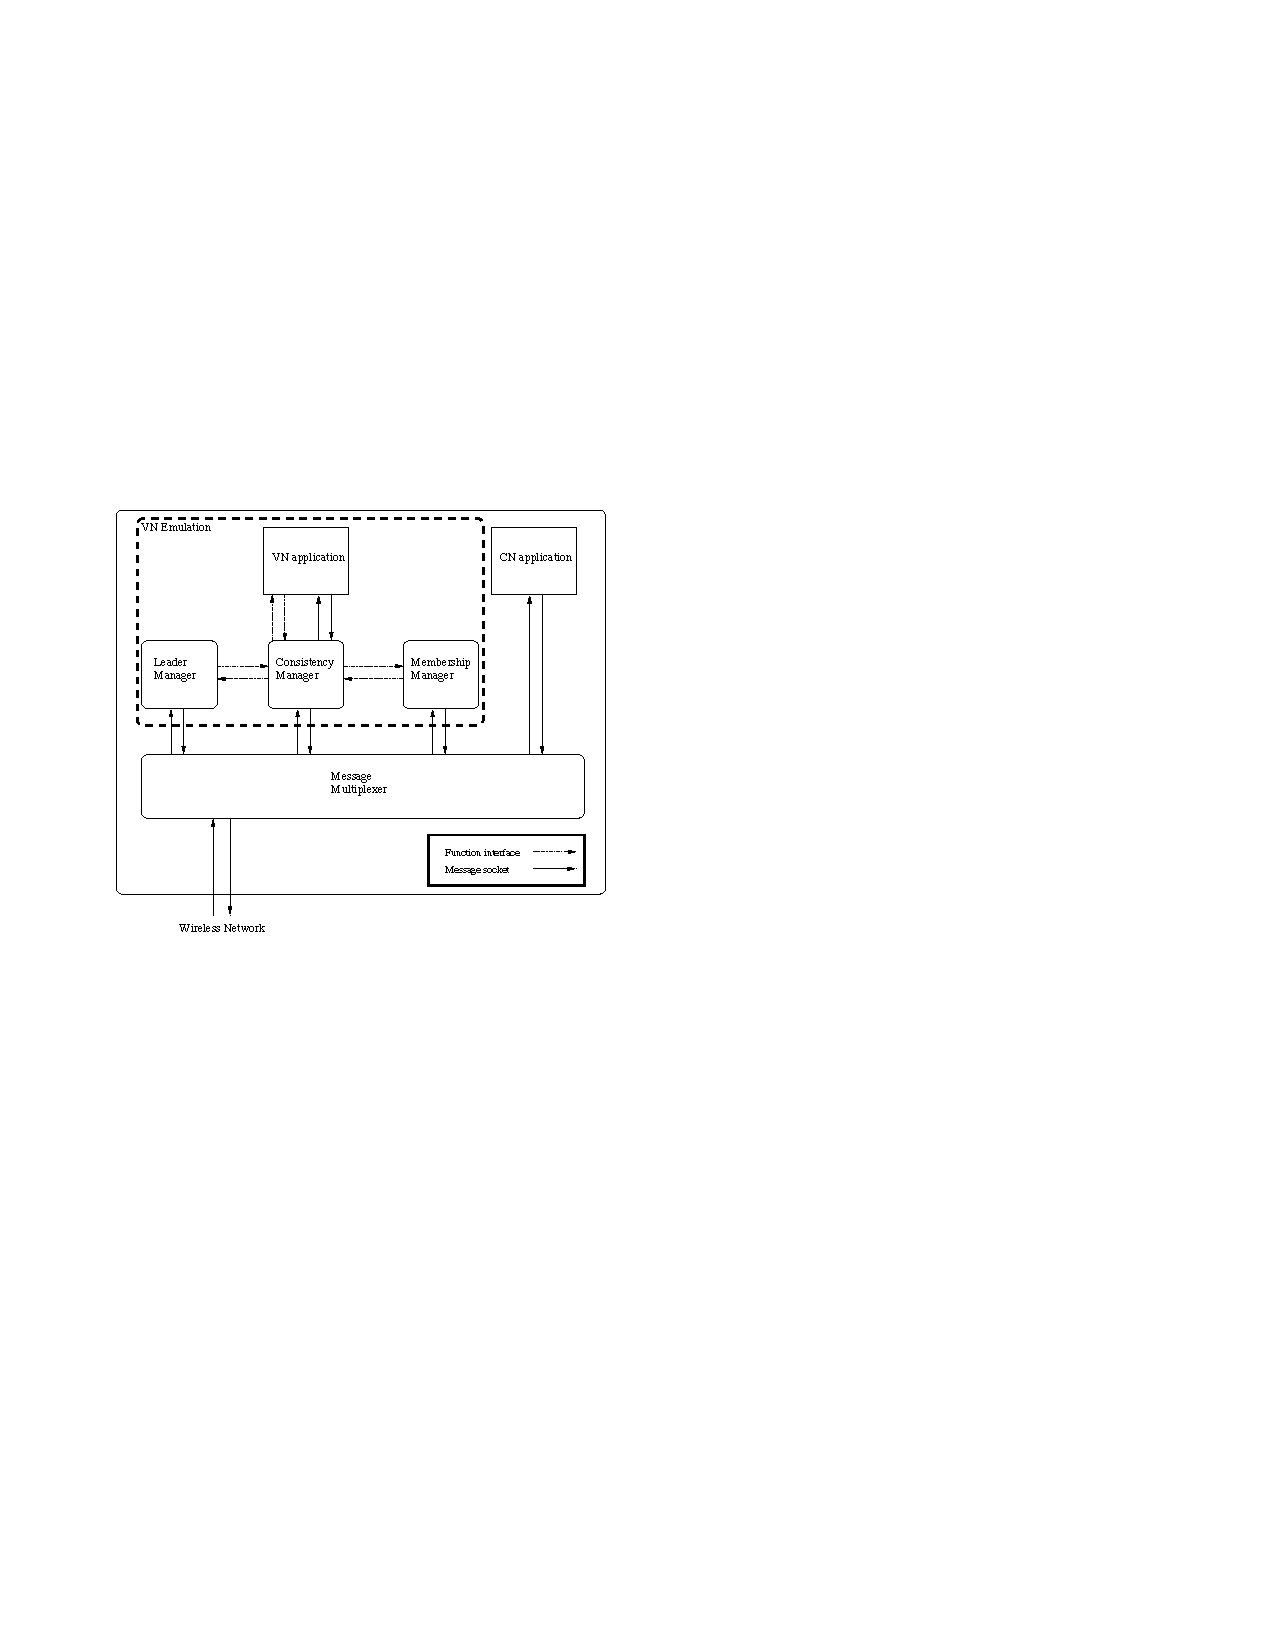
\includegraphics[width=.65\textwidth]{vnlayerarchitecture.pdf} 
\caption{VNLayer Architecture \cite{vnlayer}}
\label{fig:vnlayerArch}
\end{figure}
The VNLayer abstraction is implemented by the client nodes; this means the emulation software must maintain a consistent view of the layer.  In order to do this in a fault tolerant manner, the VN application uses  {\bf leader, consistency, and membership managers} as outlined in figure \ref{fig:vnlayerArch}.  The following is a description of the three managers and VN application:
\begin{description}
\item[Leader Manager:] Elects a leader in the region about the VN and returns  the leader status of the physical node it is running.
\item[Membership Manager:] Returns the current state or a time-out of the emulated VN application.  A time out occurs if there are no other nodes in the region about the VN.
\item[Consistency Manager:] This component is in charge of keeping the emulated VN synchronized with the physical nodes in the region. It calls upon the leadership and membership managers.\\
This component also implements the incoming and outgoing message sockets used in the VN application. 

\item[VN Application:] This implements {\em getState} and {\em updateState} functions that are called by the Consistency Manager.  $getState$ returns the VN applications current state and $updateState$ resets the state to the values passed in as parameter to the function.  
\end{description}

\subsubsection{Reactive VNLayer}
$Reactive\ VNs$ are event-driven automata: their operations occur upon receiving a message which can transform the automata state and potentially return messages to be broadcast in response.  The VNs are located at fixed, known location and fail if the region about the VN does not contain any physical nodes.  In addition, the Reactive VNLayer allows messages to be lost.  
In the Reactive VNLayer, the three managers described above have the following implementation properties: 
\begin{description}
\item[Leader Manager:] This component uses a pulse-based algorithm: the leader sends out a pulse at regular intervals.  If the pulse times out, the client node tries to declare itself as leader.  If multiple nodes are attempting to declare themselves as leader, the node with the lowest ID is selected.  \\
Due to message loss, multiple nodes might elect themselves as leader. This is handled by having any leader who hears a pulse from a  leader with a lower ID relinquish its status as leader.  
\item[Membership Manager:] This uses a simple join protocol, which asks the leader for emulated VN applications state.  If no leader exists, this request times out. 
\item[Consistency Manager:]In the Reactive VNLayer, all physical nodes emulate the VN application, but only the leader broadcasts the VN Application's messages.  
\end{description}
\subsubsection{Virtual Traffic Light}
As outlined in \cite{vnlayer}, the virtual traffic light is a possible application of the Reactive VNlayer.  We assume that each client has access to information about the time and its current location and can communicate with other clients using a local broadcast service. Then, the VN for the intersection is emulated by the CNs that are being run by the physical, autonomous cars approaching and leaving the intersection. 

The VN is programed to inform the CNs approaching the intersection the color of the traffic light in its direction.  To insure progress, the VN keeps track of the amount of time the intersection has shown a certain color.  Although the Reactive VN does not have a clock, the CNs do  (from assumption), and each time a CN sends a message it timestamps it with its clock time.  This is then used by the VN for the best estimated of the current time.   

The algorithm goes as follows:  Clients broadcast their current time, position, and heading in UPDATE messages.  The VNLayer reacts to the message in a $msgReceived$ function as shown in figure \ref{fig:vnlayerAlg}.  The VN for this application is programmed to update its state upon receiving this message and possibly change the color of some of the roads' lights based on the $UpdateLightState$ function. 

\begin{figure}
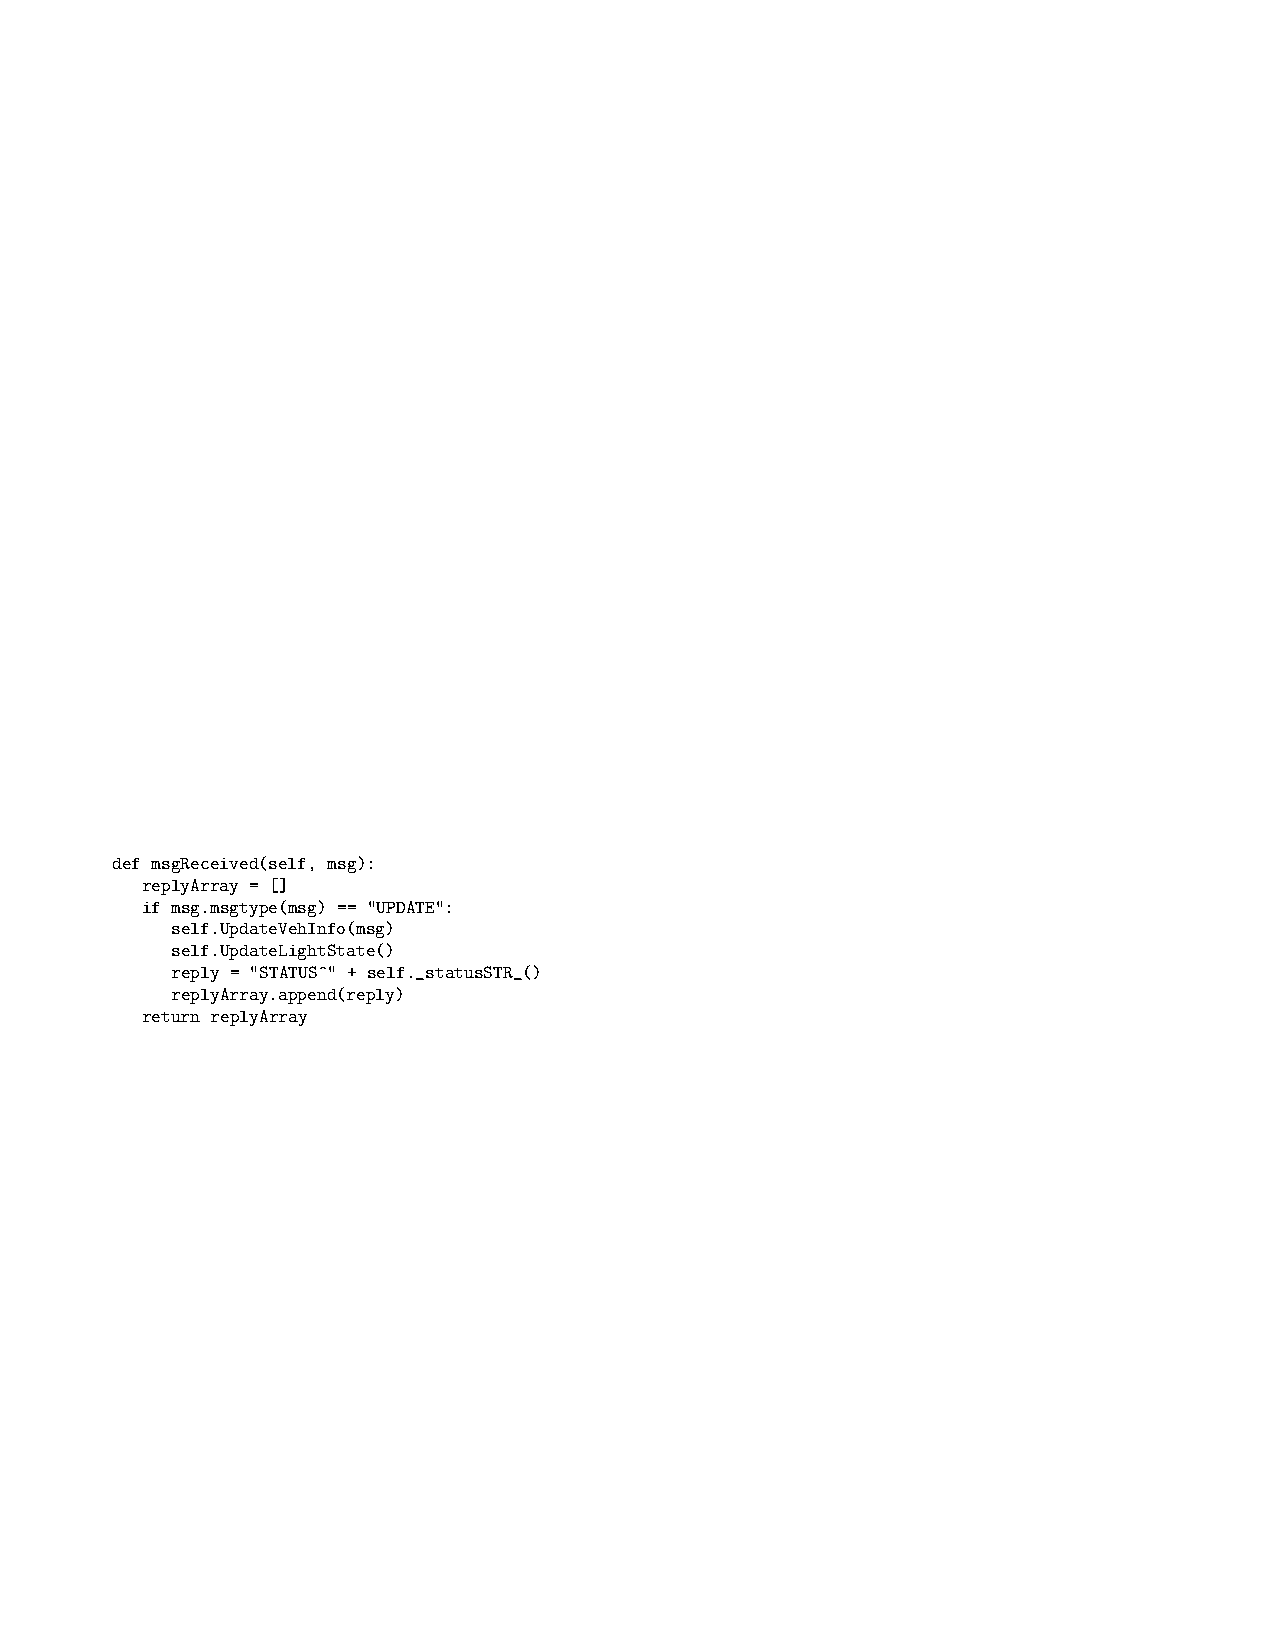
\includegraphics[width=.65\textwidth]{vnlayerAlg.pdf}
\caption{Code for the $msgReceived$ function \cite{vnlayer}}
\label{fig:vnlayerAlg}
\end{figure}
The $UpdateLightFunction$ works as follows: whenever the VN determines that a predetermined minimum "green time" has passed for the green light for a direction , or if it sees that there are no more vehicles heading in that direction, then it changes the direction's lights to yellow.  Then, once the VN sees a predetermined "yellow time" has passed it changes the direction for that light to red and the opposite direction to green.  

\subsection{Liveness and Safety Properties}
\begin{description}
\item[Safety]
 In this implementation, the following safety property is satisfied: only clients in a single direction see a non-red light.
\item[Liveness] 
 Essentially, $UpdateLightState$ works in a round robin fashion, granting green lights to populated direction in order.  This ordering insures the algorithm is fair and cars do not have to wait indefinitely to receive a green light. 
\end{description}

\subsection{Self-Stabilization}
The VNLayer has the self-stabilization property:  the ability to recover from an arbitrarily corrupt state\cite{ssvnlayer}.  Note that in the Leadership manager, the system works by pulsing messages and can elect more than one leader, which eventually gets fixed because the leader with the higher ID will relinquish its status after receiving a message from a leader with a lower ID. 
\subsection{Conclusion}
One concern with this approach is that the behavior of the stop light can be inconsistent until the VNLayer  self-stabilizes. This stoplight might work ideally in a intersection where there are always cars within the network so the VN application is consistently being emulated in a stable configuration. 
Maybe something else? %XXX Could this fail the safety property or just make vehicles wait until stabilization is achieved?
Unlike the algorithms in Section \ref{sec:tokenRing} and \ref{sec:DNF}, the traffic light application for VNLayers does not handle the extra evaluation criteria outlined in \ref{sec:problemDefinition}.  However, the abstraction to VNs and CNs makes the ability to program the application much simpler.  It is possible that messages from CNs could include more information for the $updateLightStatus$ to use.  For example, the message could include a boolean value $isAmbulance$ which the $updateLightStatus$ will use to change the light to the ambulance's direction faster than the predetermined wait time. 

\section{Future Work}
\label{sec:futureWork}
A great deal of research has focused on creating centralized autonomous intersection algorithms; this is probably due to the ease of programming of the application.  Creating a fault tolerant decentralized algorithm is nontrivial;  however, the Reactive VNLayers greatly simplifies this process.  The  centralized virtual traffic light implemented using Reactive VNLayers described in Section \ref{sec:VNLayer} could potentially be extended to implement more advanced centralized autonomous intersection algorithms.  For example, the traffic light application currently does not take into account priority of other vehicles or improving throughput,  fuel consumption, or the amount of time the cars are stopped as described in other algorithms.  However, since VNLayer allows us to emulate a centralized traffic controller, it's possible we could adapt centralized algorithms such as %XXX
to create an approach that is decentralized, but has the desired evaluation properties outlined in Section \ref{sec:problemDefinition}, in addition to the properties of the centralized algorithms it simulates.   %bla this is bad I talked about this in conclusion earlier...


\section{Conclusion}
\label{sec:conclusion}

\pagebreak

\begin{thebibliography}{9}

\bibitem{dresner}
Kurt Dresner and Peter Stone. ''Multiagent Traffic Management: An Improved Intersection
Control Mechanism", AAMAS'05 Proceedings of the fourth international joint conference on Autonomous agents and multiagent systems, New York, NY, USA, 2005.
\bibitem{naumann}
Naumann, Rolf, and Rainer Rasche. ``Intersection collision avoidance by means of decentralized security and communication management of autonomous vehicles", Univ.-GH, SFB 376, 1997.
\bibitem{tszchiu}
Au, Tsz-Chiu, Neda Shahidi, and Peter Stone. ``Enforcing Liveness in Autonomous Traffic Management." AAAI. 2011.
\bibitem{vnlayer}
Brown, Matthew, et al. "The virtual node layer: a programming abstraction for wireless sensor networks." SIGBED Review 4.3 (2007): 7-12.
\bibitem{ssvnlayer}
Nolte, Tina, and Nancy Lynch. ``Self-stabilization and virtual node layer emulations." Stabilization, Safety, and Security of Distributed Systems. Springer Berlin Heidelberg, 2007. 394-408.
\end{thebibliography}
\end{document}
